En un videojuego, la interfaz es esencial para transmitir información al jugador tanto dentro del juego para poder interactuar con dicho mundo, como en los menús para modificar elementos externos del juego tales como guardar una partida, cambiar especificaciones de la visualización del juego, etc.Por ello, en esta sección se especificará con detalle cada una de las pantallas y los menú que componen \nombrejuego. Además, se indicarán las transiciones entre ellas así como la utilidad de cada elemento de la GUI (\emph{Graphical User Interface}). Las imágenes adjuntas son bocetos que ilustran los componentes que debe contener cada pantalla, no obstante, los artistas podrán hacer cambios en la apariencia y disposición de los elementos si así lo consideran oportuno.
    
    \section{HUD (\emph{Heads-Up Display})}
    
    \label{sec:menus}
        \section{Diagrama de flujo}
        En todo juego, los menús necesitan de una jerarquía u orden a la hora de aparecer en pantalla. Para ello, normalmente se usa un diagrama que establece de manera visual el orden y la manera de cómo se puede acceder a los distintos menús durante el juego. Normalmente en un juego pequeño, dónde normalmente solo hay uno o dos menús, se puede hacer innecesario. Pero en cuanto intentemos realizar un juego que necesite de más de cuatro menús diferentes, se hace inviable el no esquematizar el orden de estos. No solo para el programador, sino para el jugador, pues el tener que ir buscando el menú específico de forma complicada, hará que dicho jugador se canse rápidamente del juego y consecuentemente abandonarlo. El siguiente diagrama de estados muesta las pantallas presentes a lo largo de \nombrejuego y las transiciones entre ellas.
        
        \begin{figure}[H] 
                \begin{center}
                    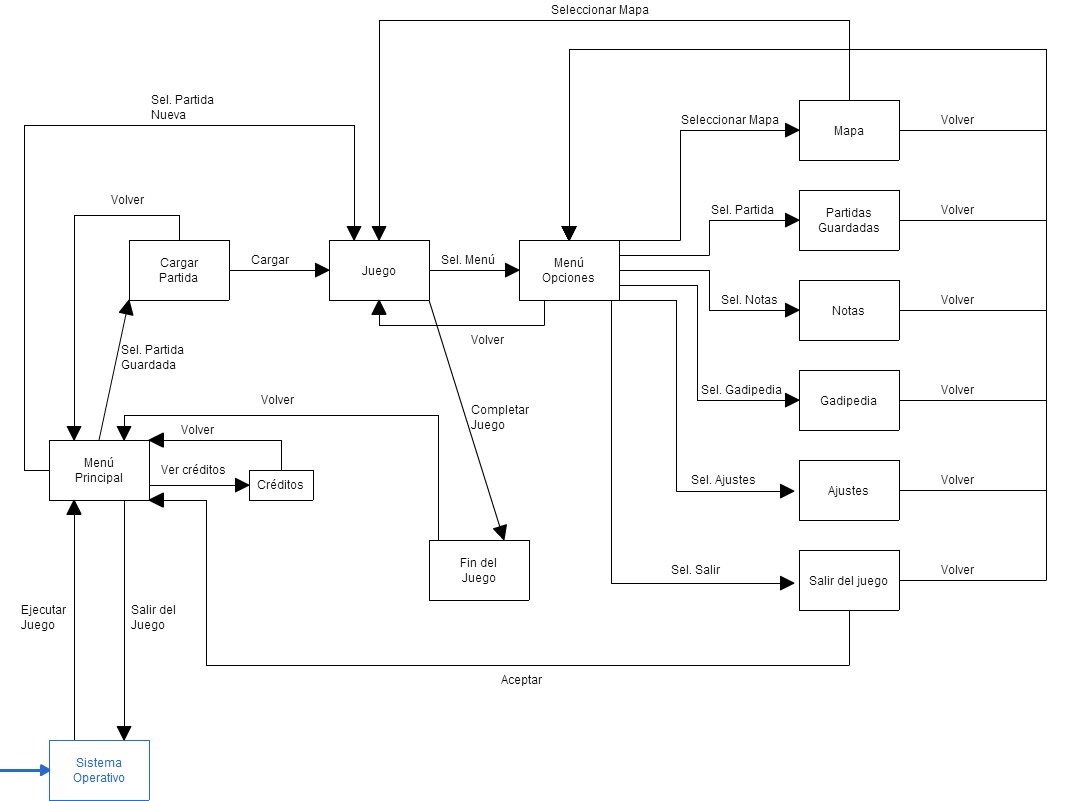
\includegraphics[scale=0.45]{diagrama_flujo_menu.png}
                \end{center}
                \caption{Diagrama de flujo de pantallas en el juego}
                \label{fig:diagrama-flujo-menu}
            \end{figure}
        
        \section{Descripciones de las pantallas}
        En esta sección nos centraremos en describir de manera individual todas las pantallas que hacen aparición en \nombrejuego.
        
        \newpage
            \subsection{Menú principal}
            A continuación el boceto de la pantalla de \emph{Menú Principal} :
            
            \begin{figure}[H] 
                \begin{center}
                    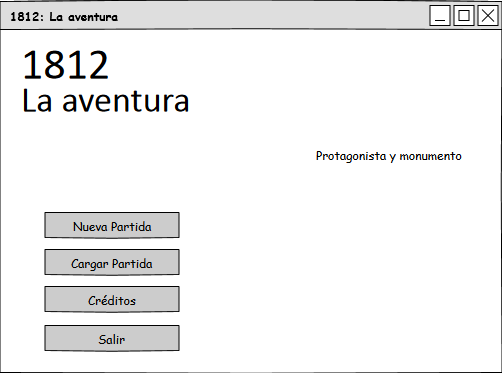
\includegraphics[scale=0.7]{men_principal.png}
                \end{center}
                \caption{Boceto del Menú Principal}
                \label{fig:menu-principal}
            \end{figure}
            
            Lista y descripción de todos sus componentes:
            \begin{itemize}
            \item \negrita{Botón Nueva Partida}: al pulsarlo lleva a la pantalla de \emph{Crear Partida}.
            \item \negrita{Botón Cargar Partida}: al pulsarlo lleva a la pantalla de \emph{Cargar Partida}.
            \item \negrita{Botón Créditos}: al pulsarlo nos lleva a la pantalla \emph{Créditos}.
            \item \negrita{Botón Salir}: al pulsarlo nos lleva de vuelta al Sistema Operativo.
            \item \negrita{Protagonista y monumento}: Una ilustración del protagonista de \nombrejuego situado en un monumento emblemático del 1812.
            \end{itemize}
            
            \newpage
            \subsection{Cargar Partida}
            A continuación el boceto de la pantalla de \emph{Cargar Partida} :
            
            \begin{figure}[H] 
                \begin{center}
                    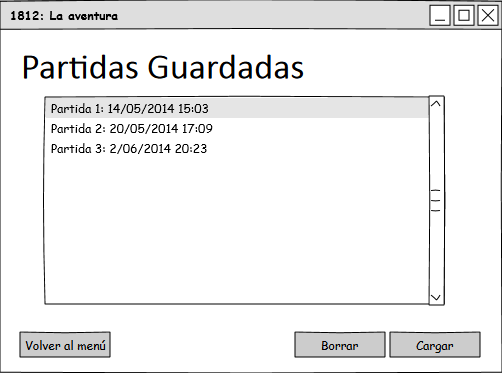
\includegraphics[scale=0.7]{cargar_partida.png}
                \end{center}
                \caption{Boceto de la pantalla de Cargar Partida}
                \label{fig:cargar-partida}
            \end{figure}
            
            Lista y descripción de todos sus componentes:
            \begin{itemize}
            \item \negrita{Lista de partidas}: lista con las partidas guardadas hasta el momento. Se muestra el día y la hora de la última actualización de esa partida.
            \item \negrita{Botón Cargar}: al pulsarlo coge la partida seleccionada y carga la pantalla de juego tal y como la dejamos.
            \item \negrita{Botón Borrar}: al pulsarlo nos dará un
            \item \negrita{Botón Volver al menú}:
            \end{itemize}
            
            \newpage
            \subsection{Créditos}
            
            
            \newpage
            \subsection{Menú Opciones}
        
        
            \newpage
            \subsection{Mapa}
            
            
            \newpage
            \subsection{Partidas guardadas dentro del juego}
            A continuación el boceto de la pantalla de \emph{Partidas Guardadas} dentro del juego :
            
            \begin{figure}[H] 
                \begin{center}
                    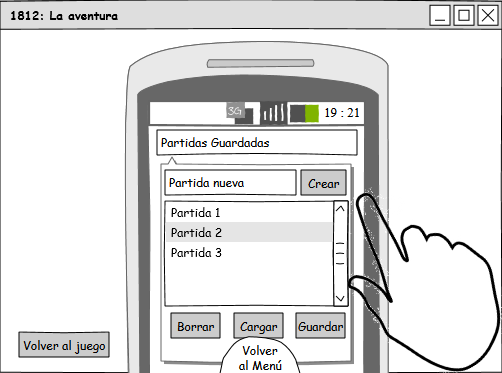
\includegraphics[scale=0.7]{cargar_partida_dentro_del_juego.png}
                \end{center}
                \caption{Boceto de la pantalla de Cargar Partida}
                \label{fig:cargar-partida-dentro-juego}
            \end{figure}
            
            Lista y descripción de todos sus componentes:
            \begin{itemize}
            \item \negrita{Crear partida nueva}: etiqueta y caja de texto para introducir el nombre de la nueva partida.
            \item \negrita{Botón Crear}: crea una nueva partida con el nombre que contiene la caja de texto. Si el perfil existe o no se ha introducido un nombre, una ventana con un mensaje aparecerá indicando el error.
            \item \negrita{Lista de partidas}: lista con las partidas guardadas hasta el momento. Se muestra el día y la hora de la última actualización de esa partida.
            \end{itemize}
            
            \newpage
            \subsection{Gadipedia}
            
            
            \newpage
            \subsection{Notas}
            
            
            \newpage
            \subsection{Ajustes}
            
            
            \newpage
            \subsection{Salir}
        %\subsection{Trucos y \emph{Easter Eggs}}
        %Por ahora no hay intención de introducir trucos y \emph{Easter Eggs}.